\documentclass[11pt]{article}

\usepackage[utf8]{inputenc}
\usepackage[T1]{fontenc}
\usepackage{lmodern}
\usepackage{geometry}
\usepackage{graphicx}
\usepackage{booktabs}
\usepackage{microtype}
\IfFileExists{xurl.sty}{\usepackage{xurl}}{\usepackage{url}}
\IfFileExists{bookmark.sty}{\usepackage{bookmark}}{}
\usepackage[round,authoryear]{natbib}
\usepackage{hyperref}
\usepackage{caption}
\usepackage{float}
\IfFileExists{balance.sty}{\usepackage{balance}}{}

\newif\ifhasticz
\IfFileExists{tikz.sty}{
  \hasticztrue
  \usepackage{tikz}
  \usetikzlibrary{arrows.meta,calc,positioning}
}{
  \hasticzfalse
}

\geometry{margin=1in}

\hypersetup{
  colorlinks=true,
  linkcolor=black,
  citecolor=black,
  urlcolor=black,
  pdftitle={Learning Without Curriculum: How Students Learn Technical Skills Outside Formal Education},
  pdfauthor={Ruthwik Reddy}
}

\emergencystretch=2em
\sloppy

\setlength{\parindent}{0pt}
\setlength{\parskip}{0.6em}
\setlength{\intextsep}{0.8em}
\setlength{\textfloatsep}{1.0em}
\setlength{\floatsep}{0.8em}

\captionsetup{font=small,labelfont=bf}

\IfFileExists{enumitem.sty}{
  \usepackage{enumitem}
  \setlist{nosep}
}{}

\title{Learning Without Curriculum: How Students Learn Technical Skills Outside Formal Education}
\author{Ruthwik Reddy\\Independent Student Researcher}
\date{2026}

\begin{document}

\maketitle

\begin{abstract}
Traditional pedagogical models emphasize linear, curriculum-based instruction as the primary pathway for technical skill acquisition. However, an increasing demographic of "student builders" acquires complex competencies through independent, problem-driven execution. This paper presents an analytic auto-ethnographic study of these curriculum-independent learning trajectories, drawing on a longitudinal dataset of technical artifacts, version control histories, and personal documentation from 2021 to 2026. The study identifies a recursive "Need--Build--Validate" loop as the foundational mechanism of skill construction. Within this framework, skill acquisition is triggered by situated technical needs, developed through hands-on implementation, and validated by functional outcomes and community feedback. Furthermore, the study examines the role of generative Artificial Intelligence (G-AI) as a bounded scaffold in modern learning workflows. The findings offer a critical perspective on educational design, credentialing, and the evolving nature of technical expertise in an AI-integrated landscape.
\end{abstract}

\onecolumn
\tableofcontents
\clearpage
\twocolumn

\section{Introduction}

Curriculum-based education remains the dominant framework for teaching technical skills in schools and universities. These systems emphasize predefined learning outcomes, linear topic sequencing, and assessment through examinations or grades. While effective for standardized instruction, such models often fail to account for learners who acquire skills through real-world problem solving, project execution, and iterative failure outside formal classrooms.

In recent years, the rise of accessible online documentation, open-source ecosystems, and AI-assisted learning tools has enabled students to bypass traditional instructional pathways entirely. Many student builders now learn programming, system design, and product development not because a syllabus requires it, but because a real problem demands it. Despite the visibility of this phenomenon, academic literature has largely focused on structured self-learning platforms \citep{chen2023} or maker education programs, rather than deeply examining independent, curriculum-free learning trajectories.

This paper addresses that gap by asking: \textbf{How do independent student builders construct and validate technical skills without a formal curriculum?} By grounding the analysis in lived experience rather than abstract theory, the study aims to make informal, real-world learning academically legible.

\section{Related Work}

Research on self-directed learning (SDL) has long emphasized learner autonomy, intrinsic motivation, and metacognitive regulation \citep{knowles1975,zimmerman2002}. The SDL framework identifies three foundational processes: motivational (maintaining commitment), metacognitive (planning and monitoring progress), and applied (implementing strategies and reflecting on outcomes). Contemporary research confirms that SDL skills can be systematically developed through assessment, evaluation, planning, monitoring, and adjustment cycles---a framework equally applicable to formal and informal contexts.

More recent studies in problem-based learning (PBL) highlight the power of authentic problem triggers in initiating learning \citep{hmelo2004}. Research demonstrates that effective triggers---problems designed with strategic clues and connection to real-world scenarios---produce significantly better learning outcomes than conventional instruction. Additionally, studies emphasize the role of ``trigger design'': problems should stimulate real-life engagement, encourage knowledge integration, fit learners' prior knowledge, and generate learning issues aligned with meaningful objectives.

Portfolio and project-based assessment has emerged as a valid alternative to traditional testing \citep{lam2021}. These methods show superior outcomes: companies using project-based technical evaluations report 40\% reductions in employee turnover and 50\% improvements in identifying high-performing talent. Unlike standardized tests, project-based evaluation measures technical accuracy, problem-solving approach, code quality, and communication---a more holistic assessment.

The alternative credentials movement has expanded significantly, with micro-credentials, digital badges, and competency-based assessment gaining institutional recognition \citep{gallagher2022}. These credentials are performance-based (earned through demonstrated mastery, not grades) and stackable (modular qualifications that combine into larger certifications). Prior Learning Assessment (PLA) programs, such as the Council for Adult and Experiential Learning's (CAEL) Learning Counts, now provide pathways to formally recognize skills acquired outside traditional education.

Perspectives from constructionist and maker-oriented learning further support the centrality of building as a pathway to understanding, where learners construct knowledge through meaningful projects rather than passively receiving content \citep{papert1980,resnick2017}.

Finally, open-source communities represent a parallel learning infrastructure in which practices, norms, and peer feedback act as informal curriculum and assessment; this ecosystem-level view aligns with accounts of how open collaboration produces knowledge and expertise \citep{raymond1999}.

However, most existing studies examine learning within semi-structured environments---MOOCs, bootcamps, or school-supported maker spaces. Few investigate fully independent learners operating without instructional scaffolding, external grading, or formal credential requirements. This study contributes a longitudinal, artifact-based analysis of curriculum-independent technical learning over multiple years, addressing the ``why'' alongside the ``how'' of skill acquisition.

\section{Methodology}

\subsection{Research Design}

To investigate the mechanisms of complex skill acquisition in non-formal environments, this study utilizes an \textit{analytic auto-ethnographic} framework \citep{ellis2011}. Auto-ethnography allows for a systematic analysis of personal experience to illuminate broader cultural and technical phenomena. By treating the researcher as the primary unit of observation, this method provides granular access to internal motivations, cognitive triggers, and the iterative "wrestling" with technical systems that is often obscured in large-scale quantitative studies.

This longitudinal analysis covers technical projects and learning trajectories from 2021 to 2026, a period coinciding with the emergence of generative AI as a fundamental component of the developer ecosystem.

\subsection{Data Sources}

The analysis is grounded in a triangulation of several primary data streams:

\begin{enumerate}
\item \textbf{Technical Artifacts}: Production-level codebases, architectural prototypes, and functional web applications (e.g., IdeaBoard, WorkScape).
\item \textbf{Version Control Metadata}: Granular Git histories that document the temporal expansion of codebases, iterative refactorings, and the introduction of new dependencies.
\item \textbf{Heuristic Documentation}: Design specifications, reflective dev-logs, and community discussions (e.g., GitHub issues, Discord threads).
\item \textbf{Longitudinal Skill Maps}: Reconstructed timelines correlating specific technical barriers with the subsequent acquisition of prerequisite competencies.
\end{enumerate}

Validation in this context is defined by \textit{functional efficacy} and \textit{community adoption} rather than standardized metrics, aligning with professional software engineering norms.

\begin{figure}[t]
\centering
\ifhasticz
\makebox[\linewidth][c]{\resizebox{\linewidth}{!}{%
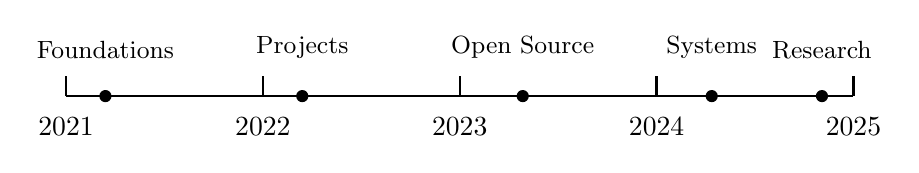
\begin{tikzpicture}[x=1cm,y=1cm]
  \draw[thick] (0,0) -- (10,0);
  \foreach \x/\y in {0/2021,2.5/2022,5/2023,7.5/2024,10/2025} {
    \draw[thick] (\x,0) -- (\x,0.25);
    \node[anchor=north] at (\x,-0.15) {\y};
  }
  \foreach \x/\label in {0.5/Foundations,3/Projects,5.8/Open\ Source,8.2/Systems,9.6/Research} {
    \fill (\x,0) circle (2.2pt);
    \node[align=center,anchor=south,font=\small] at (\x,0.35) {\label};
  }
\end{tikzpicture}%
}}%
\else
\fbox{\parbox[c][0.22\textheight][c]{0.95\linewidth}{\centering Figure placeholder}}
\fi
\caption{Learning Milestones of an Independent Student Builder (2021--2025).}
\end{figure}

\subsection{Data Analysis: Thematic Coding and Reflexivity}

The data was categorized through a thematic coding process focused on trigger mechanisms, learning modes, and validation cycles. Analysis followed an iterative inductive approach, where emerging patterns were continuously tested against the technical artifacts. Key dimensions included:

\begin{itemize}
\item \textbf{Trigger Identification}: Classifying the impetus for learning (e.g., architectural failure, competition-driven deadlines).
\item \textbf{Mechanism Correlation}: Mapping the relationship between the identified need and the subsequent learning mode (e.g., documentation synthesis vs. reverse-engineering).
\item \textbf{Validation Evaluation}: Analyzing the social and functional signals that confirmed competency acquisition.
\end{itemize}

\subsection{Positionality and Reflexivity}

In auto-ethnographic research, the researcher’s positionality is a critical factor. As a student builder deeply embedded in developer communities, I possess "insider" knowledge that allows for a nuanced reading of technical artifacts. To mitigate potential bias toward self-affirmation, I practiced active reflexivity—purposefully seeking evidence of failures, cognitive shortcuts, and instances where independent learning proved inefficient compared to formal instruction.

\section{Findings}

The analysis indicates that learning without a curriculum is a non-random, structured process revolving around a recursive \textbf{Need--Build--Validate} loop. Competencies are acquired when a situated technical need arises, implemented through hands-on project execution, and validated by the functional and social performance of the resulting artifacts.

\subsection{Skill Acquisition Triggers: The "Need" Mechanism}

The study identified five primary trigger mechanisms that initiate learning trajectories. Rather than following a predefined syllabus, skill acquisition is driven by authentic challenges encountered during production.

\subsubsection{Problem-Driven Triggers}

The majority of learning episodes were initiated by specific technical barriers or "walls." For example, the acquisition of React was not the result of formal instruction but was necessitated by the requirement for a dynamic user interface in a specific web application. In this model, the problem serves as the pedagogical catalyst, reversing the traditional classroom sequence where theory precedes application.

\subsubsection{Deadline-Driven Triggers}

External and internal temporal constraints served as significant motivators. Competitions, project launch dates, and self-imposed deadlines forced a prioritization of essential concepts, encouraging a "pragmatic deep dive" into the most critical documentation and implementation patterns.

\subsubsection{Failure-Driven Triggers}

Deeper conceptual understanding often emerged from system failures. Architectural breakdowns and cryptographic errors provided fertile ground for investigations into underlying principles. For instance, a Cross-Site Scripting (XSS)—a security vulnerability allowing malicious scripts to be injected into websites—necessitated a rigorous study of JSON Web Tokens (JWT) and Cross-Origin Resource Sharing (CORS) policies. Similarly, a PostgreSQL deadlock led to an investigation into transaction isolation levels and query optimization; and recurring Docker memory failures prompted an analysis of container orchestration and resource management. In these cases, the failure acted as a "diagnostic trigger" for advanced theoretical learning.

\subsubsection{Experimentation-Driven Triggers}

A subset of learning episodes was driven by exploratory curiosity. While not always tied to a production deadline, these technical experiments built a "latent toolkit" of competencies that could be mobilized when a production-level problem later emerged.

\subsubsection{Community-Driven Triggers}

Social standards and peer expectations also functioned as learning catalysts. Observing high-quality open-source architectures and receiving feedback on code contributions established "competency benchmarks" that the learner aimed to replicate.

\textbf{Key Finding}: These triggers represent \textit{situated, authentic, and self-identified} learning prompts, aligning with theories of legitimate peripheral participation \citep{lave1991}.

\begin{figure}[t]
\centering
\ifhasticz
\makebox[\linewidth][c]{\resizebox{\linewidth}{!}{%
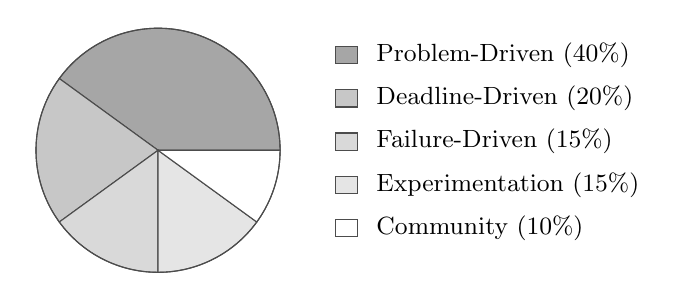
\begin{tikzpicture}[x=1cm,y=1cm,font=\small]
  \def\R{1.55}
  \def\cx{0}
  \def\cy{0}
  \tikzset{slice/.style={draw=black!70,thin}}
  \tikzset{leg/.style={anchor=west,font=\small}}

  % Segments (40/20/15/15/10) -> angles (144/72/54/54/36)
  \def\aA{0}
  \def\aB{144}
  \def\aC{216}
  \def\aD{270}
  \def\aE{324}
  \def\aF{360}

  \path[slice,fill=black!35] (\cx,\cy) -- (\aA:\R) arc (\aA:\aB:\R) -- cycle;
  \path[slice,fill=black!22] (\cx,\cy) -- (\aB:\R) arc (\aB:\aC:\R) -- cycle;
  \path[slice,fill=black!15] (\cx,\cy) -- (\aC:\R) arc (\aC:\aD:\R) -- cycle;
  \path[slice,fill=black!10] (\cx,\cy) -- (\aD:\R) arc (\aD:\aE:\R) -- cycle;
  \path[slice,fill=white]     (\cx,\cy) -- (\aE:\R) arc (\aE:\aF:\R) -- cycle;
  \draw[slice] (\cx,\cy) circle (\R);

  % Legend
  \def\lx{2.25}
  \def\ly{1.10}
  \def\sw{0.28}
  \def\sh{0.22}
  \fill[black!35] (\lx,\ly) rectangle (\lx+\sw,\ly+\sh);
  \draw[black!70,thin] (\lx,\ly) rectangle (\lx+\sw,\ly+\sh);
  \node[leg] at (\lx+0.40,\ly+0.11) {Problem-Driven (40\%)};

  \fill[black!22] (\lx,\ly-0.55) rectangle (\lx+\sw,\ly-0.55+\sh);
  \draw[black!70,thin] (\lx,\ly-0.55) rectangle (\lx+\sw,\ly-0.55+\sh);
  \node[leg] at (\lx+0.40,\ly-0.55+0.11) {Deadline-Driven (20\%)};

  \fill[black!15] (\lx,\ly-1.10) rectangle (\lx+\sw,\ly-1.10+\sh);
  \draw[black!70,thin] (\lx,\ly-1.10) rectangle (\lx+\sw,\ly-1.10+\sh);
  \node[leg] at (\lx+0.40,\ly-1.10+0.11) {Failure-Driven (15\%)};

  \fill[black!10] (\lx,\ly-1.65) rectangle (\lx+\sw,\ly-1.65+\sh);
  \draw[black!70,thin] (\lx,\ly-1.65) rectangle (\lx+\sw,\ly-1.65+\sh);
  \node[leg] at (\lx+0.40,\ly-1.65+0.11) {Experimentation (15\%)};

  \fill[white] (\lx,\ly-2.20) rectangle (\lx+\sw,\ly-2.20+\sh);
  \draw[black!70,thin] (\lx,\ly-2.20) rectangle (\lx+\sw,\ly-2.20+\sh);
  \node[leg] at (\lx+0.40,\ly-2.20+0.11) {Community (10\%)};
\end{tikzpicture}%
}}%
\else
\fbox{\parbox[c][0.22\textheight][c]{0.95\linewidth}{\centering Figure placeholder}}
\fi
\caption{Breakdown of Learning Triggers (2021--2025). ``Problem-Driven'' is the most common, highlighting the importance of authentic challenges.}
\end{figure}

\subsection{Non-Linear Skill Construction: Rejecting the Linear Syllabus}

Predictably, curriculum-independent learning does not follow a linear, hierarchical sequence. Instead, it manifests as a "messy," non-linear progression consisting of three primary patterns.

\subsubsection{Just-in-Time Learning (JITL)}

Skill acquisition occurs primarily on an "as-needed" basis. The learner may master a specific library or architectural pattern to resolve an immediate barrier, which may then remain untouched for extended periods. This Just-in-Time Learning (JITL) approach creates a profile of deep but narrow competencies, contrasting with the "broad but shallow" foundations of traditional introductory curricula.

\subsubsection{Concurrent Multi-Skill Development}

The study observed the simultaneous acquisition of disparate technical skills within a single project cycle. For instance, the development of a full-stack application required the concurrent learning of frontend frameworks, backend runtimes, database schemas, and deployment orchestration. This multidisciplinarity reflects real-world software engineering contexts better than modularized educational units.

\subsubsection{Reverse-Engineering as a Foundational Mode}

A significant portion of learning was derived from the deconstruction of existing systems. Rather than studying algorithms in abstraction, the learner derived principles by analyzing functional codebases. This "learning-by-doing in reverse" provides a high-fidelity model of how software systems are integrated in practice.

\begin{figure}[t]
\centering
\ifhasticz
\makebox[\linewidth][c]{\resizebox{\linewidth}{!}{%
\begin{tikzpicture}[x=1cm,y=1cm,>=Latex,font=\small]
  \tikzset{nodebox/.style={draw,black!70,thick,rounded corners,fill=black!8,align=center,minimum width=4.2cm,minimum height=1.05cm}}

  \node[nodebox] (jit) at (0,0) {Just-in-Time\\Learning};
  \node[nodebox] (cms) at (5.2,0) {Concurrent\\Multi-Skill};
  \node[nodebox] (re)  at (2.6,-2.0) {Reverse-\\Engineering};

  \draw[->,black!70,thick] (jit) -- (cms);
  \draw[->,black!70,thick] (cms) -- (re);
  \draw[->,black!70,thick] (re) -- (jit);
\end{tikzpicture}%
}}%
\else
\fbox{\parbox[c][0.22\textheight][c]{0.95\linewidth}{\centering Figure placeholder}}
\fi
\caption{Patterns of Non-Linear Skill Acquisition.}
\end{figure}

\subsection{Validation Without Grades: The Performance of Competence}

In the absence of formal assessment, skill validation is derived from functional and social signals. The study identified four primary mechanisms through which competence was verified.

\subsubsection{Functional Outcomes as Primary Proof}

The primary validation signal was simply the operational success of the artifact. The ability to build a functioning system that resolves a specific problem serves as an objective measure of competence, often carrying more weight in developer communities than standardized test scores.

\subsubsection{User Adoption and Feedback}

External validation occurred when artifacts were adopted by others. Bug reports, feature requests, and user engagement provided a "market-based" validation of the learner's technical and product-design competencies.

\subsubsection{Peer Review and Contribution Acceptance}

Acceptance into open-source repositories functioned as a rigorous validation mechanism. Having contributions reviewed and merged by experienced maintainers serves as a strong signal of professional-level competence, mirroring the feedback loops found in expert-led tutoring \citep{schmidt1995}.

\subsubsection{Public Portfolios as Credentialing Infrastructure}

The maintenance of a public version-control profile (e.g., GitHub) functions as a dynamic credential. Unlike static certificates, a portfolio demonstrates continuous skill application and growth over time, aligning with theories of networked and community-situated learning \citep{ito2013}.

\textbf{Key Finding}: Unlike episodic classroom assessments, validation in this model was \textbf{continuous, multi-faceted, and externally driven}.

\begin{figure}[t]
\centering
\ifhasticz
\makebox[\linewidth][c]{\resizebox{\linewidth}{!}{%
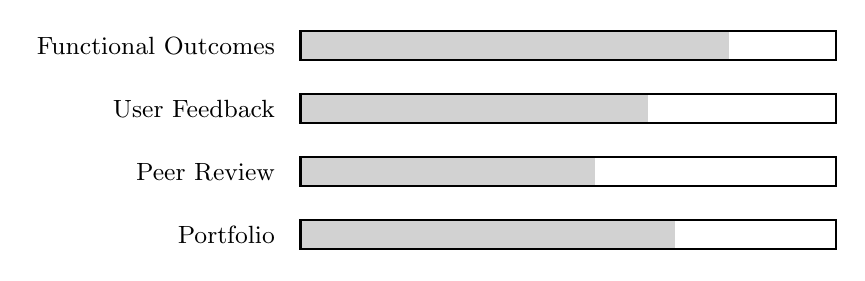
\begin{tikzpicture}[x=1cm,y=1cm]
  \def\w{6.8}
  \foreach \y/\label/\val in {0.0/Functional Outcomes/0.80, -0.8/User Feedback/0.65, -1.6/Peer Review/0.55, -2.4/Portfolio/0.70} {
    \node[anchor=east,font=\small] at (0,\y) {\label};
    \fill[gray!35] (0.2,\y-0.18) rectangle ({0.2+\w*\val},\y+0.18);
    \draw[thick] (0.2,\y-0.18) rectangle ({0.2+\w},\y+0.18);
  }
\end{tikzpicture}%
}}%
\else
\fbox{\parbox[c][0.22\textheight][c]{0.95\linewidth}{\centering Figure placeholder}}
\fi
\caption{Methods of Skill Validation.}
\end{figure}

\subsubsection{Functional Outcomes as Proof}

The most important validation was simple: did it work? If I could build a web app that people could use, or a tool that solved a real problem, that was the proof. It is a direct measure of competence compared to a test score.

\subsubsection{User Feedback and Adoption}

When people started using the things I built, their feedback was a powerful form of validation. Bug reports, feature requests, and even positive comments showed that work was having impact.

\subsubsection{Peer Code Review and Contribution Acceptance}

In open source, having your code reviewed and accepted by other developers is a rigorous validation mechanism. When a contribution is merged, it is a strong signal of competence, similar in spirit to the feedback processes described in tutoring and guided learning environments \citep{schmidt1995}.

\subsubsection{Public Portfolio Demonstration}

Everything I’ve built is on my GitHub. This public portfolio functions as a credential because it shows what I can do, not just what courses I’ve taken. This aligns with broader accounts of learning that is socially networked and shaped by participation in communities \citep{ito2013}.

\textbf{Key Finding}: Unlike grades (often one-time), validation was \textbf{continuous, multi-faceted, and driven by the outside world}. Working projects and external feedback are difficult to fake.

\subsection{The Need--Build--Validate Loop}

When I put all these findings together, I saw a clear pattern: a recursive loop I call the Need--Build--Validate loop.

\begin{enumerate}
\item \textbf{Need}: It starts with a trigger---a problem, a deadline, a failure, curiosity, or the community---creating a need to learn something new.
\item \textbf{Build}: I learn the skill by building something, using documentation, AI tools, and community resources.
\item \textbf{Validate}: The thing I built provides validation. If it works, if people use it, and if other developers respect it, then I know I’ve learned the skill.
\end{enumerate}

\begin{figure*}[t]
\centering
\ifhasticz
\makebox[\textwidth][c]{\resizebox{\textwidth}{!}{%
\begin{tikzpicture}[x=1cm,y=1cm,>=Latex]
  \node[draw,rounded corners,minimum width=3.5cm,minimum height=1.1cm,align=center,fill=gray!10] (need) at (0,0) {Need};
  \node[draw,rounded corners,minimum width=3.5cm,minimum height=1.1cm,align=center,fill=gray!10] (build) at (6,0) {Build};
  \node[draw,rounded corners,minimum width=3.5cm,minimum height=1.1cm,align=center,fill=gray!10] (validate) at (3,-2.1) {Validate};
  \draw[->,thick] (need) -- (build);
  \draw[->,thick] (build) -- (validate);
  \draw[->,thick] (validate) -- (need);
\end{tikzpicture}%
}}%
\else
\fbox{\parbox[c][0.18\textheight][c]{0.95\textwidth}{\centering Figure placeholder}}
\fi
\caption{The Need--Build--Validate Learning Loop.}
\end{figure*}

The key is that this isn't a one-time process. Every finished project opens new possibilities and new problems, which starts the loop again.


\subsection{AI-Assisted Learning: The 2025--2026 Context}

The rise of generative AI (G-AI) development tools has become a primary factor shaping how independent builders acquire and refine technical skills. Unlike previous generations of online resources, G-AI tools such as Gemini, ChatGPT, and Claude function as interactive scaffolds that can compress the time between a technical question and a verifiable implementation \citep{bakker2024}.

\subsubsection{Documentation Acceleration}

AI tools reduce search and synthesis time by providing immediate, context-aware summaries of APIs, error messages, and implementation patterns. This increases momentum during the "Build" phase of the loop by allowing the learner to iterate quickly on hypotheses. For example, when encountering complex state management patterns or cryptic TypeScript errors, Claude and Gemini can break down system-level issues into manageable conceptual steps. However, research suggests that this perceived speed must be balanced against the need for independent verification to avoid shallow skill acquisition \citep{bakker2024}.

\subsubsection{Validation Through AI-Generated Feedback}

AI systems increasingly function as high-fidelity "review partners," approximating the role of a human mentor for solo learners. By flagging potential bugs, suggesting refactors, and proposing test cases, AI tools provide intermediate validation before a project reaches the community or production stages. This aligns with recent findings on the utility of AI-generated feedback in student co-creation processes, where timely, automated critiques support iterative improvement without the bottlenecks of human review \citep{pozdniakov2025}.

\subsubsection{Responsible AI Usage as a Meta-Skill}

The effective orchestration of AI systems is itself a significant learned capability. This shifts technical competence toward prompt formulation, output verification, and the ability to detect "stochastic hallucinations" \citep{bender2021}. Mastering these meta-skills is essential for ensuring that AI-assisted learning supports rather than simplifies the cognitive wrestling required for expertise.

\subsubsection{Risks and Cognitive Failure Modes}

Despite its benefits, AI-assisted learning introduces significant risks that can erode the quality of learning if left unaddressed.

\begin{enumerate}
\item \textbf{Hallucinations and Credibility Risks.} Models can generate confident but fabricated citations or explanations. In research contexts, this necessitates a "verify first" protocol where all AI-generated claims are grounded in primary sources.
\item \textbf{Workflow Fragility.} Over-reliance on specific AI models creates dependency. Technical learning must remain tool-agnostic to survive changes in access or model behavior.
\item \textbf{The Illusion of Competence.} AI can produce working code without requiring the learner to internalize the underlying logic. This "cognitive outsourcing" can lead to skill atrophy and a failure to transfer knowledge to novel problems \citep{ericsson1993,bakker2024}.
\end{enumerate}

These risks imply that AI should be used as a \textbf{bounded scaffold} rather than a substitution for foundational understanding, especially in academic and high-stakes technical environments.


\section{Discussion}

The recursive \textbf{Need--Build--Validate} model offers a significant framework for understanding the mechanisms of technical skill acquisition outside formal institutions. By triangulating theories of self-directed learning \citep{knowles1975,zimmerman2002}, problem-based learning \citep{hmelo2004}, and constructionism \citep{papert1980}, the model demonstrates how the intrinsic demands of technical production serve as a high-fidelity alternative to traditional curricula.

\subsection{Theoretical Implications}

The study highlights a direct tension between static academic curricula and dynamic technical ecosystems. While formal programs provide foundational breadth, they often lack the temporal agility to keep pace with rapid shifts in software engineering (e.g., the transition to G-AI development). Curriculum-independent learning, by contrast, is inherently "agile," responding quickly to the immediate requirements of the technical environment.

However, the analysis also identifies a critical trade-off in "Just-in-Time" learning cycles. While the learner acquires deep, production-ready expertise in specific domains, they may bypass foundational concepts (e.g., database normalization or algorithmic complexity) if those concepts are not immediately necessitated by the artifact being built. This suggests that while curriculum-independent learning excels at technical \textit{performance}, it may require purposeful supplementation to ensure architectural \textit{depth}.

\subsection{Implications for Educational Design}

The findings suggest several avenues for the evolution of formal technical education:

\begin{enumerate}
\item \textbf{Inversion of the Pedagogical Sequence}: Rather than theory-first instruction, programs should adopt a "problem-first" approach where theoretical concepts are introduced as secondary scaffolds for active project implementation.
\item \textbf{High-Fidelity Artifact Assessment}: Institutional evaluation should shift toward professional-grade artifacts—codebases, version-control histories, and peer-reviewed contributions—which provide a more accurate signal of competency than standardized examinations \citep{lam2021}.
\item \textbf{AI-Integrated Scaffolding}: Educational design must treat AI as a learned capability, focusing on prompt architecture, output verification, and the prevention of shallow "cognitive outsourcing."
\end{enumerate}

\subsection{Implications for Credentialing}

As learning pathways diversify, industry and academia must develop recognition mechanisms that capture competencies achieved through independent execution:

\begin{enumerate}
\item \textbf{Portfolio-Based Signaling}: Public, longitudinal artifacts (e.g., GitHub profiles) serve as high-signal credentials that demonstrate both technical proficiency and a history of self-directed growth.
\item \textbf{Micro-Credentialing for Modular Skill-Sets}: Organizations should recognize modular, performance-based certifications that validate specific competencies acquired through Just-in-Time Learning (JITL) \citep{gallagher2022}.
\item \textbf{Community-Validated Expertise}: Signals from developer communities—such as pull-request acceptance into major open-source projects—should be academically and professionally legible.
\end{enumerate}

\subsection{Limitations and Future Research}

As an auto-ethnographic study, the generalizability of these findings is bounded by the researcher’s specific socio-technical context, motivation level, and access to resources. Future research should prioritize multi-subject studies to examine how the Need--Build--Validate loop operates across diverse backgrounds and domains (e.g., hardware engineering, data science).

Furthermore, the long-term impact of generative AI on cognitive development remains an urgent area for investigation. Longitudinal studies are needed to determine whether AI scaffolding facilitates faster expertise development or, conversely, leads to the erosion of foundational debugging and problem-solving skills.

\section{Conclusion}

Curriculum-independent learning is not merely a supplementary practice but a robust alternative for high-motivation technical skill acquisition. The \textbf{Need--Build--Validate} loop describes a cycle where situative technical challenges trigger deep learning, implementation produces production-ready competence, and functional success provides continuous validation. While the integration of generative AI expands access and velocity, it demands a new set of meta-competencies focused on verification and scholarly rigor. Ultimately, bridging the gap between independent building and formal recognition is essential for supporting the next generation of technical innovators in an increasingly decentralized learning landscape.

\IfFileExists{balance.sty}{\balance}{}
\bibliographystyle{plainnat}
\bibliography{references}

\end{document}
